\documentclass[10pt, t]{beamer}
\usetheme{Boadilla}
\usepackage[utf8]{inputenc}
\usepackage{amsmath}
\usepackage{amsfonts}
\usepackage{amssymb}
\usepackage{graphicx}
\usepackage{gensymb}
\usepackage{ragged2e}
\usepackage{amsmath}
\usepackage{amssymb}
\usepackage{amsthm}
\usepackage{amsfonts}
\usepackage{braket}

%TODO
%Cambiare immagine iniziale che si vedono i battimenti
%TODO
%Cambiare simbolo di sommatoria
%TODO
%Verificare he si vedano bene le scritte sui grafici

\title{Anderson localization in optical lattices}
\author[Federico Belliardo]{Federico Belliardo\\{\small Relatore: Davide Rossini}}
\institute{Università di Pisa}
\date{29 Giugno 2017}

\begin{document}

\begin{frame}
\titlepage
\end{frame}

%Introduzione all'esperimento di Inguscio
%e motivazione per lo studio di Aubry-André
\begin{frame}[t]

\begin{center}
\begin{figure}
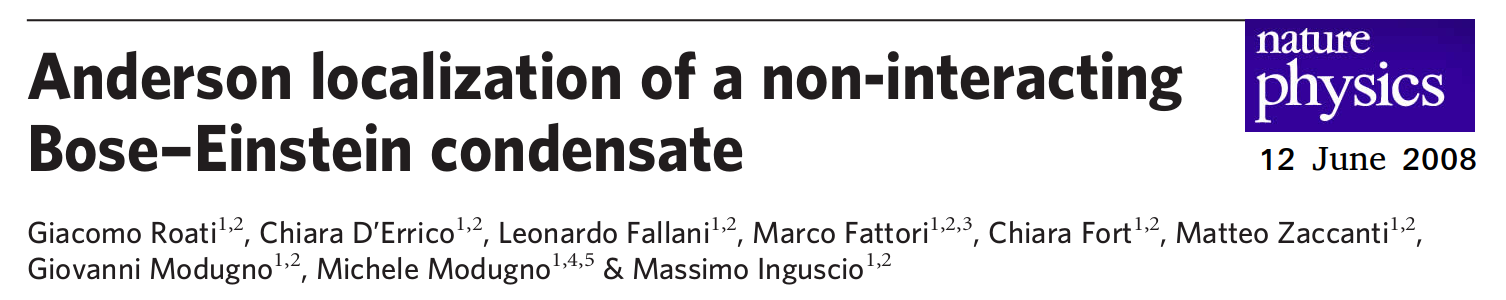
\includegraphics[scale=0.2]{immaginiPresentazione/intro.png}
\end{figure}
\end{center}
\vskip-2em
\begin{columns}
\column{0.5\textwidth}
\begin{center}
Esperimento di \emph{quantum simulation}.
$\mathcal{H} = \frac{p^2}{2 m} + A_1 \cos(k_1 x) +  A_2 \cos(k_2 x)$.
$ A_2 \ll A_1$, $k_1$ e $k_2$ \textbf{incommensurabili}.
Riconducibile al modello di Aubry-André che presenta uno \textbf{pseudo-disordine}.
\end{center}

\vskip-1em

\begin{figure}
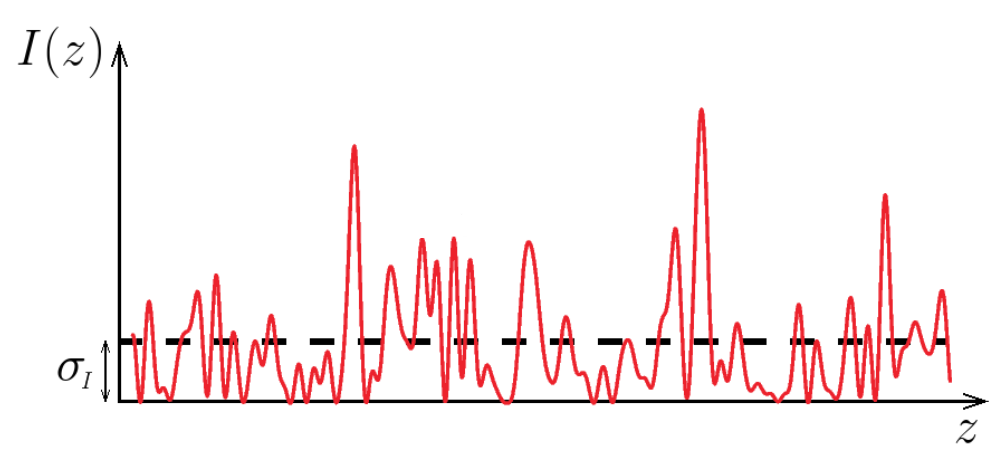
\includegraphics[scale=0.17]{immaginiPresentazione/lattice.png}
\end{figure}

\column{0.5\textwidth}

\begin{figure}
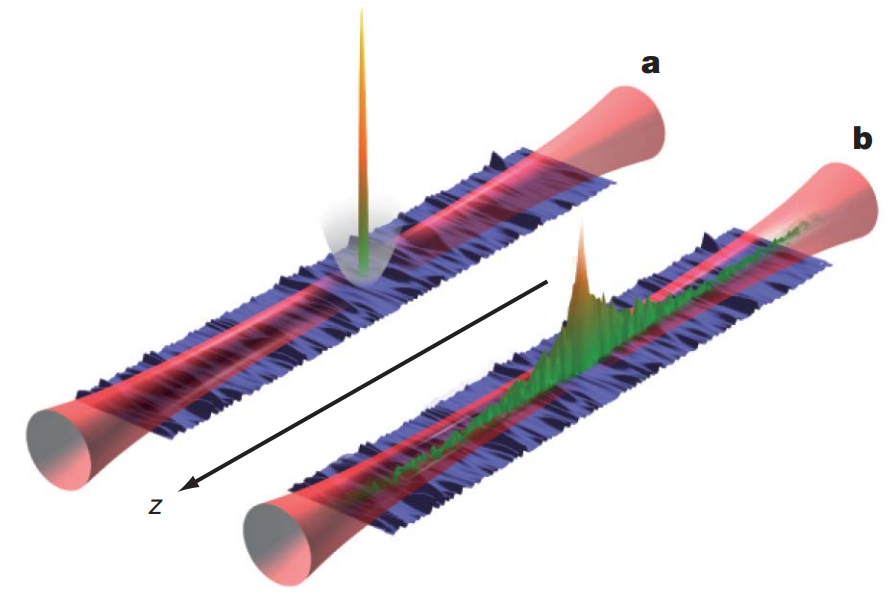
\includegraphics[scale=0.15]{immaginiPresentazione/Incipit.png}
\end{figure}


\begin{center}
Si parla di \emph{disorder induced localization}: gli autostati sono \textbf{esponenzialmente localizzati}. Esperimento simile nel gruppo di A. Aspect a Parigi (2008).
\end{center}
\end{columns}
\end{frame}


%Slide sulla dualità
\begin{frame}
\frametitle{Aubry-André self-duality}

\begin{center}

\begin{large}
$\mathcal{H} = \Delta \sum_{n=0}^{N-1} cos(2 \pi \beta n) a_n ^{\dagger} a_n + J \sum_{n=0}^{N-1} (a_{n+1}^{\dagger} a_n + a_n ^{\dagger} a_{n+1})$
\end{large}

\vspace{10pt}

%$\Delta$: intensità del disordine, $j$: termine di \emph{hopping}, $\beta = \frac{k_1}{k_2}$ è \textbf{irrazionale}. In trasformata di Fourier $a_n = \frac{1}{\sqrt{N}} \sum_{m=0}^{N-1} e^{i 2 \pi \beta n m} \tilde{a}_m$ si ottiene:

In trasformata di Fourier $a_n = \frac{1}{\sqrt{N}} \sum_{m=0}^{N-1} e^{i 2 \pi \beta n m} \tilde{a}_m$:

\vspace{10pt}

\begin{large}
$\mathcal{H} = 2 J \sum_{n=0}^{N-1} cos(2 \pi \beta n) \tilde{a}_n^{\dagger} \tilde{a}_n + \frac{\Delta}{2} \sum_{n=0}^{N-1} (\tilde{a}_{n+1}^{\dagger} \tilde{a}_n + \tilde{a}_{n}^{\dagger} \tilde{a}_{n+1})$
\end{large}

\vspace{10pt}

%Uno stesso autostato $\Ket{\psi}$ di $\mathcal{H}$ con energia $E$ localizzato su pochi siti nello spazio reale è autostato esteso dell'Hamiltoniana duale (simile alle onde di Bloch).


\textbf{Esteso $\leftarrow$ $\Ket{\psi}$ $\rightarrow$ Localizzato}

\vskip-1em

\begin{columns}
\column{0.4\textwidth}

\begin{center}
\begin{figure}
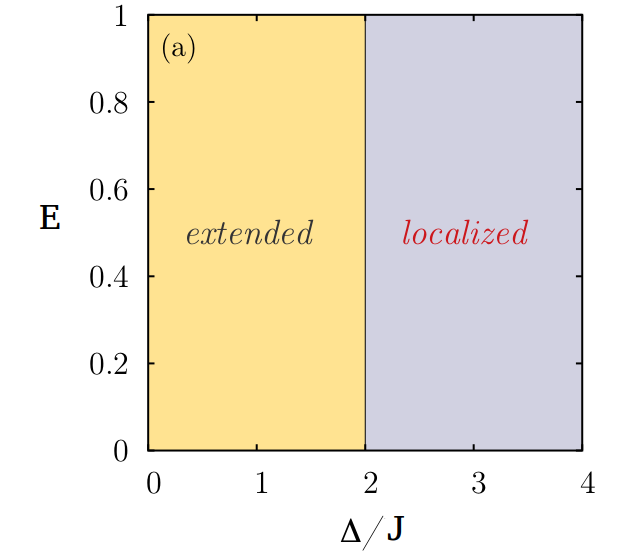
\includegraphics[scale=0.22]{immaginiPresentazione/duale.png}
\end{figure}
\end{center}

\column{0.3\textwidth}

\begin{center}
%\justifying
%Nei limiti $\Delta \rightarrow \infty$ e $\Delta \rightarrow 0$ gli stati devono essere tutti rispettivamente localizzati e estesi indipendentemente dall'energia. Si ipotizza che a $\frac{\Delta}{j} = 2$ avvenga una \emph{quantum phase transition} tra i due regimi. Non è detto che sia unica e che non vi sia un \emph{mobility edge}.

%Si ipotizza che a $\frac{\Delta}{j} = 2$ avvenga una \emph{quantum phase transition} tra i due regimi di stati localizzati e estesi. Non è detto che sia unica e che non vi sia un \emph{mobility edge}.

\vspace{20pt}
\begin{large}
$\frac{\Delta}{J} = 2$\\
\downarrow \\
Quantum phase transition
\end{large}
\end{center}
\end{columns}
\end{center}

\end{frame}

%Formula di Thouless
\begin{frame}

\frametitle{Calcolo della lunghezza di decadimento}

\begin{center}

\textbf{Formula di Thouless}: $\frac{1}{\ell_{\beta}} = \int \rho (E) \ln \left| \frac{E_{\beta} - E}{J} \right| dE$

%Ricavata supponendo per i coefficienti $c^{\beta}_n$ nello schema del \emph{tight-binding} un decadimento esponenziale: $c_1^{\beta} = e^{-\frac{|1-i|}{\ell_{\beta}}}$ e $c_N^{\beta} = e^{-\frac{|N-i|}{\ell_{\beta}}}$.%

Dalla dualità: $\frac{1}{\ell_{\beta}} = \frac{1}{\ell^{*}_{\beta}} + \ln \left( \frac{\Delta}{2 J} \right)$. Se lo stato duale è esteso otteniamo la formula per la dimensione spaziale dell'autostato:\\
\vspace{10pt}
\begin{large}
$\frac{1}{\ell_{\beta}} = \ln(\frac{\Delta}{2 J})$
\end{large}\\
\vspace{10pt}
Indipendente dall'energia. 
Le simulazioni forniscono l'\emph{inverse participation ratio}: $IPR_{\beta} = \frac{\sum_{n=0}^{N-1} |c^{\beta}_n|^4}{\sum_{n=0}^{N-1} |c^{\beta}_n|^2}$.



\begin{columns}
\column{0.4\textwidth}
\vskip-1em
\begin{figure}
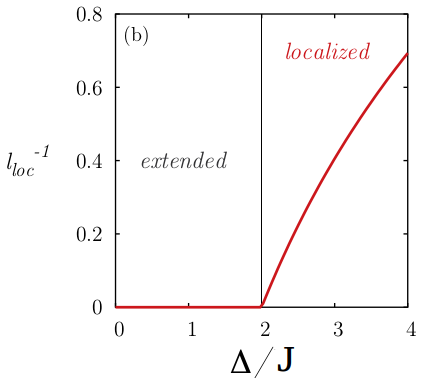
\includegraphics[scale=0.25]{immaginiPresentazione/loc.png}
\end{figure}
\column{0.4\textwidth}
\vskip-1em
\begin{figure}
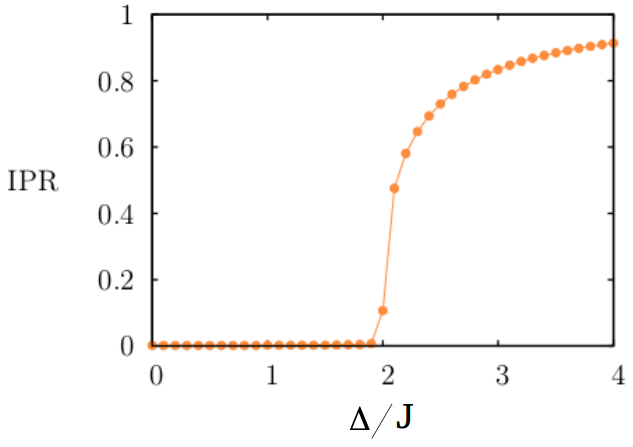
\includegraphics[scale=0.20]{immaginiPresentazione/ipr.png}
\end{figure}
\end{columns}
\end{center}
\end{frame}


\begin{frame}

\frametitle{Misure sul condensato e simulazioni}

\begin{columns}

\column{0.5\textwidth}

\begin{center}
Simulazione del profilo di densità di uno stato centrato nell'origine al variare del disordine. 
\end{center}

\begin{center}
\begin{figure}
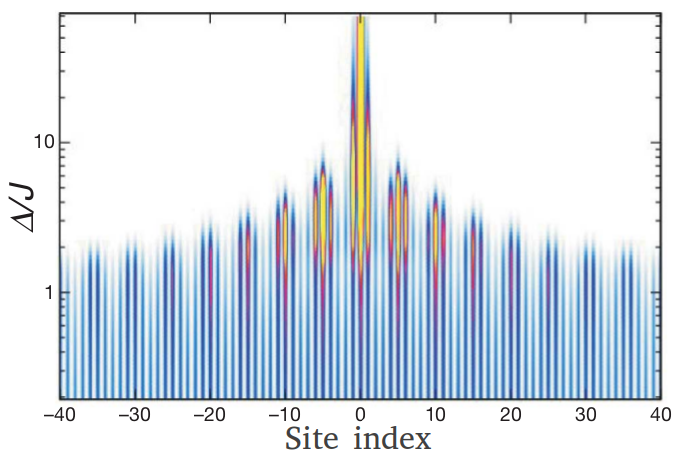
\includegraphics[scale=0.25]{immaginiPresentazione/simulation.png}
\end{figure}
\end{center}


\column{0.4\textwidth}

\begin{figure}
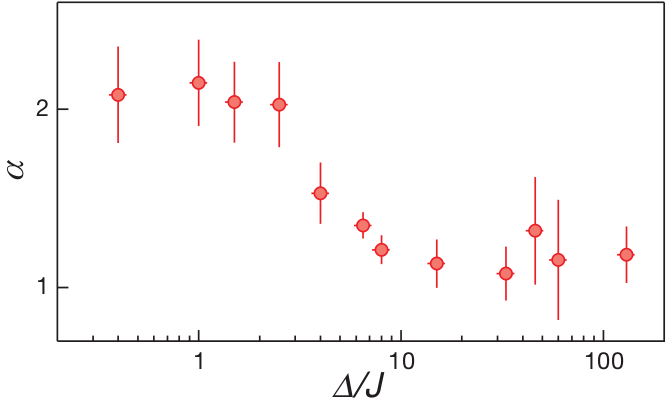
\includegraphics[scale=0.20]{immaginiPresentazione/fit1.png}
\end{figure}

\begin{center}
Il condensato non termalizza nell'espansione ma interviene il \emph{dephasing}.
Fit del profilo di densità:\\
\vspace{10pt}
$f(x) = e^{- \left| \frac{x-x_0}{l} \right| ^ {\alpha}}$
\end{center}


\end{columns}
\end{frame}

\begin{frame}

\frametitle{Misure sul condensato}
\vskip-2em

\begin{columns}

\column{0.4\textwidth}

\begin{center}

\begin{figure}
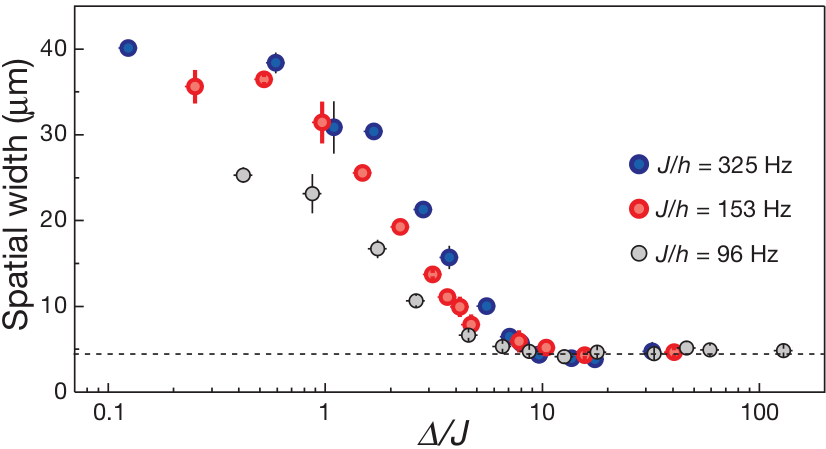
\includegraphics[scale=0.18]{immaginiPresentazione/fit2.png}
\end{figure}

\vspace{10pt}

Prima osservazione diretta della \textbf{localizzazione di Anderson}!



Oggi (2017) si studia il ruolo delle interazioni nella localizzazione (\emph{Many body localization}).
\end{center}
\column{0.5\textwidth}
\begin{center}

L'unico parametro rilevante per la transizione di fase è $\frac{\Delta}{J}$.

\begin{figure}
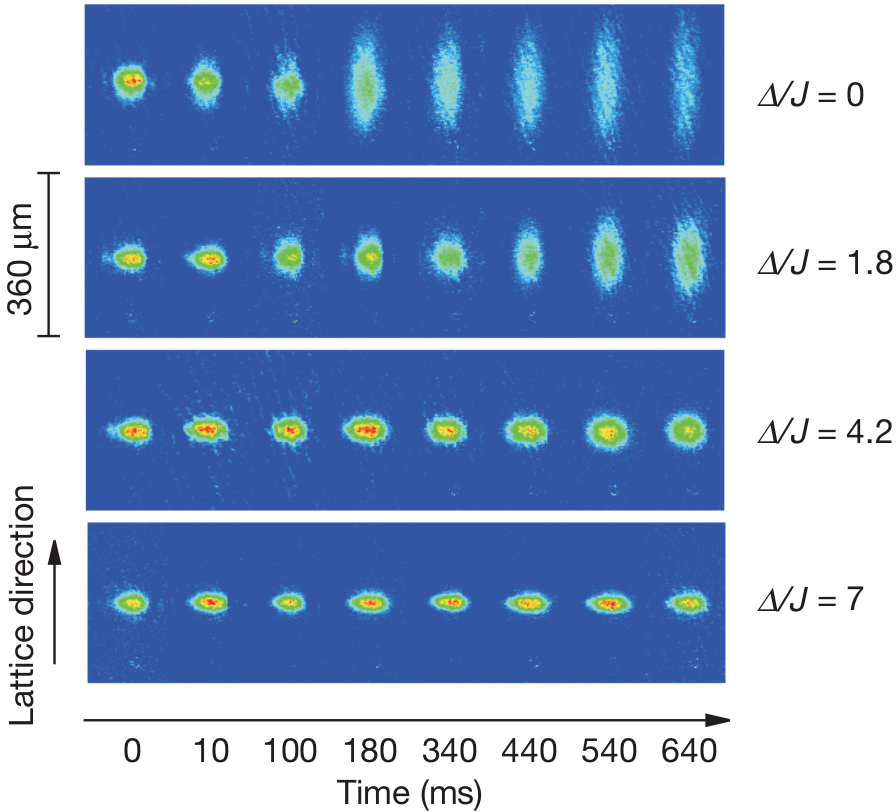
\includegraphics[scale=0.20]{immaginiPresentazione/fotoCondensato.png}
\end{figure}

\end{center}
 
\end{columns}
\end{frame}


\begin{frame}
\frametitle{Bibliografia}
\begin{itemize}
\item Anderson, P. W. \emph{Absence of diffusion in certain random 
lattices}. Phys. Rev. 109, 1492–1505 (1958).
\item Thouless D. 1972, \emph{A relation between the density of states and range of localization for one dimensional random systems}, J. Phys. C: Solid State Phys. 5 77.
\item Modugno M. \emph{Exponential localization in one-dimensional quasi-periodic optical lattices}, 2009 New J. Phys. 11 033023.
\item G. Roati et al., \emph{Anderson localization of a non-interacting Bose-Einstein condensate}, NATURE 453, 895 (12 June 2008).
\item Billy J. et al., \emph{Direct observation of Anderson localization of matter waves in a controlled disorder}, NATURE 453, 891, (12 June 2008).

\end{itemize}

\begin{center}
\textbf{Grazie per l'attenzione!}
\end{center}
\end{frame}

\end{document}
